\documentclass[a4paper]{report}
\usepackage[]{graphicx}
\usepackage[]{color}
\usepackage{alltt}
\usepackage[T1]{fontenc}
\usepackage[utf8]{inputenc}
\setcounter{secnumdepth}{3}
\setcounter{tocdepth}{3}
\setlength{\parskip}{\smallskipamount}
\setlength{\parindent}{0pt}
\usepackage{multirow}
\usepackage{tabularx}
\usepackage{fontawesome5}
\usepackage{minted}
\usemintedstyle{manni}
\usepackage[nottoc,notlot,notlof]{tocbibind}

\usepackage[x11names]{xcolor}
% Set page margins
\usepackage[top=80pt,bottom=80pt,left=68pt,right=66pt]{geometry}

% Prevents LaTeX from filling out a page to the bottom
\raggedbottom

% Adding both languages
\usepackage[english, italian]{babel}

% All page numbers positioned at the bottom of the page
\usepackage{fancyhdr}
\fancyhf{} % clear all header and footers
\fancyfoot[C]{\thepage}
\renewcommand{\headrulewidth}{0pt} % remove the header rule
\pagestyle{fancy}

% Changes the style of chapter headings
\usepackage{titlesec}
\titleformat{\chapter}
   {\normalfont\LARGE\bfseries}{\thechapter.}{1em}{}
% Change distance between chapter header and text
\titlespacing{\chapter}{0pt}{-20pt}{2\baselineskip}

% Adds table captions above the table per default
\usepackage{float}
\floatstyle{plaintop}
\restylefloat{table}

% Adds space between caption and table
\usepackage[tableposition=top]{caption}
% Adds hyperlinks to references and ToC
\usepackage{hyperref}
\hypersetup{hidelinks,linkcolor = black} % Changes the link color to black and hides the hideous red border that usually is created

% If multiple images are to be added, a folder (path) with all the images can be added here 
\graphicspath{ {figures/} }

\definecolor{wizard}{HTML}{1B3F91}

\setminted{breaklines,xleftmargin=20pt,linenos,frame=lines,framesep=2mm}
%%%%%%%%%%%%%%%%%%%%%%%%%%%%%% Starts the document
\begin{document}
\sffamily

%%% Selects the language to be used for the first couple of pages
\selectlanguage{italian}

\newgeometry{top=100pt,bottom=100pt,left=68pt,right=66pt}
%%%%% Adds the title page
\begin{titlepage}
	\clearpage\thispagestyle{empty}
	\centering
	\vspace{1cm}

	{\LARGE Corso di Programmazione Web e Mobile \\ 
		A.A. 2022-2023 \par}
		\vspace{3cm}
	{\bfseries\Huge WizardGuard \\ \vskip0.1cm}
    \noindent\textcolor{wizard}{\rule{10cm}{1.5mm}}\\
    {\LARGE \url{https://wizardguard.org} \\ \vskip0.1cm}
	\vspace{3.6cm}
	{\Large Michele Castoldi -- 893291 \\
	        Alessandro Fontana -- 20540A \par}
	\vspace{3cm}
    
    \centering 
\includegraphics[scale=0.4]{wizardguard}
    
    \vspace{2.6cm}
		
	% Set the date
	\raggedright{\normalsize Autori: Michele Castoldi, Alessandro Fontana \\Ultima modifica: \today{} -- versione 1.0.0 \\
    Prima modifica: 10 ottobre 2023 \par}
	
	\pagebreak

\end{titlepage}

\restoregeometry

% Adds a table of contents
\tableofcontents



\chapter{Introduzione}\label{chapt:sum}
WizardGuard è un servizio multipiattaforma per la conservazione sicura e relativa gestione di login (username, password e MFA), carte di pagamento e note.

Il focus principale del progetto è cercare di garantire un buon livello di sicurezza all'utente finale, per farlo ci siamo basati sul sistema di crittografia end-to-end utilizzato da Bitwarden Inc., il noto password mananger open source \cite{bitwarden}.

Le tecnologie utilizzate sono: Node.js per il backend, HTML5, CSS e Javascript per il frontend, MongoDB per la persistenza dei dati e Apache Cordova per l'applicazione Android.

\section{Breve analisi dei requisiti}
\subsection{Destinatari}
Il target di riferimento è rappresentato da chiunque abbia la necessità di organizzare le proprie credenziali di accesso in maniera sicura, centralizzata e accessibile, pertanto la forbice d'età risulta molto ampia, non essendo oltretutto richieste competenze tecniche avanzate.

L'attuale modello implementativo non si rivolge all'ambito aziendale, in cui è richiesta una gestione gerarchica degli utenti e la possibile condivisione (con regole e vincoli) delle credenziali immagazzinate.

Per facilitare l'esperienza d'uso degli utenti, le funzionalità sono espresse con una interfaccia visiva intuitiva, corredata da messaggi di testo guidati e indicazioni d'uso. Inoltre vi è stata una scelta mirata nei colori e nelle regole d'uso degli stessi (es. bottoni di conferma, eliminazione) per garantire coerenza ed evitare confusione.

\subsection{Motivazione}
Le motivazioni che possono spingere un utente ad utilizzare l’applicazione possono essere molteplici:
\begin{itemize}
\item \textbf{organizzative}: considerando la quantità di credenziali che oggi anche un utente base del web deve avere, l'organizzazione in maniera puntuale e centralizzata nonché accessibile da dispositivi differenti;
\item \textbf{sicurezza informatica}: un utente con una spiccata sensibilità per la sicurezza online e l'importanza di una corretta gestione di credenziali e dati personali;
\item \textbf{psicologiche}: la consapevolezza di demandare la scelta (rispettando i requisti richiesti) e la conservazione delle password ad un applicativo crittografato e sicuro rende l'utente più tranquillo nell'approcciarsi alla navigazione web.
\end{itemize}
Il livello di motivazione è attivo, in quanto l'uso di tale applicazione è dettato da un'esigenza/volontà dell'utente.

Rifacendoci al modello di Bates identifichiamo una tipologia di ricerca mirata delle informazioni (attiva e diretta).

\subsection{Modello di valore}
L’applicazione e i servizi ad essa collegati sono erogati in modalità gratuita agli utenti.

Si pensano modelli di business che potranno essere supportati in futuro:
\begin{itemize}
    \item \textbf{Freemium (ambito utente privato)}: l'applicativo potrà prevedere l'introduzione di piani d'uso (uno gratuito e uno a pagamento) con funzionalità differenti. In particolare introducendo nel piano gratuito limiti nelle credenziali salvabili nella cassaforte digitale, superati nel piano a pagamento. In più si prevede l'esclusività di alcune funzionalità per il solo piano a pagamento (es. report periodici di verifica di credenziali e carte di pagamento compromesse, condivisione sicura degli elementi ed importazione/esportazione della propria cassaforte);
    \item \textbf{Affiliazione (ambito utente privato)}: l'utente di qualsiasi piano avrà la possibilità di condividere un link di affiliazione personale che potrà essere utilizzato da nuovi utenti in fase di registrazione. Nel caso in cui venga sottoscritto il piano a pagamento tramite il link di affiliazione, entrambi gli utenti coinvolti riceveranno dei benefit. L'utente affiliante con piano gratuito riceve la possibilità di fare l'upgrade al piano a pagamento per un periodo limitato di tempo. L'utente affiliante con piano a pagamento e l'utente affiliato, ricevono uno sconto sul rinnovo del piano;
    \item \textbf{Sottoscrizione (ambito aziendale)}: si prevede l'implementazione delle funzionalità richieste in ambito aziendale (gestione gerarchica degli utenti e la possibile condivisione, con regole e vincoli, delle credenziali immagazzinate) sottoscrivibili tramite vari piani a pagamento dipendenti dal numero di utenti amministrati.
\end{itemize}

\section{Flusso dei dati}
Il flusso dei dati risulta generato dagli utenti che ne hanno completa autonomia nella gestione. Per garantire l'accesso da più dispositivi, i dati dell'utente vengono archiviati in modo criptato e inaccessibile, se non dall'utente stesso, in un database. Considerato il modello di lavoro dell'applicativo, il valore dello stesso è costituito dal numero di utenti attivi, rispetto ai dati a loro collegati.

Sui dati verranno applicati i concetti di privacy e security by design (solo le informazioni necessarie verranno salvate sul database) e by default (ogni utente ha accesso alle sole informazioni da lui inserite).

\section{Aspetti tecnologici}
L'applicativo si compone di 3 elementi principali:
\begin{itemize}
    \item \textbf{frontend}: l'interfaccia, condivisa tra sito web e applicazione mobile, è scritta in HTML5 e CSS con l'ausilio del framework Bootstrap\cite{bootstrap}. La logica applicativa è sviluppata in Javascript mediante l'utilizzo di jQuery\cite{jquery}. Le dipendenze sono incluse tramite NPM\cite{npm} e compilate mediante Browserify\cite{browserify}, permettendo quindi una gestione più semplice e rapida degli aggiornamenti.
    \item \textbf{backend}: le REST API sono sviluppate da un server NodeJS\cite{nodejs} con framework Express\cite{express}. Le API permettono la gestione degli utenti, delle sessioni ad essi associate e della cassaforte personale mediante la messa a disposizione di una serie di endpoint di chiamata. Per gestire le interazioni con il database si fa uso del framework mongoose\cite{mongoose}. Le dipendenze sono gestite tramite NPM.
    \item \textbf{database}: database NoSQL MongoDB\cite{mongo} per l'archiviazione persistente dei dati degli utenti.
\end{itemize}
\section{Infrastruttura}
Si descrivono le scelte infrastrutturali messe in opera per la pubblicazione dell'applicativo.

Per ricondurre il progetto ad un prodotto reale abbiamo registrato un dominio (wizardguard.org) così da rendere accessibile il client web.

Per il frontend web si è provveduto a sfruttare il servizio cloud Render\cite{render}, che mette a disposizione in maniera gratuita la pubblicazione di uno static site tramite un server http Node.js. Sfruttando le impostazioni messe a disposizione da Render si è provveduto a configurare, con specifici record DNS, la base uri del dominio di progetto.

Simile soluzione è stata adottata per il backend, il quale è stato reso accessibile su un dominio di terzo livello dedicato (api.wizardguard.com).

Il database è stato pubblicato sul servizio DBaaS Atlas offerto da MongoDB Inc. e risulta accessibile tramite uno specifico indirizzo di host e credenziali di accesso (username e password).

Il codice di frontend e backend è pubblicato su due differenti e dedicati repository Git\cite{git}, ospitati su GitHub\cite{github}, da cui Render acquisisce automaticamente i sorgenti da pubblicare.

Per l'invio delle mail agli utenti è stato configurato opportunamente un account Zoho\cite{zoho}, che offre un server SMTP gratuito, associabile al proprio dominio.

\section{Funzionamento del sistema di cifratura}
    \begin{figure}[H]
        \centering
        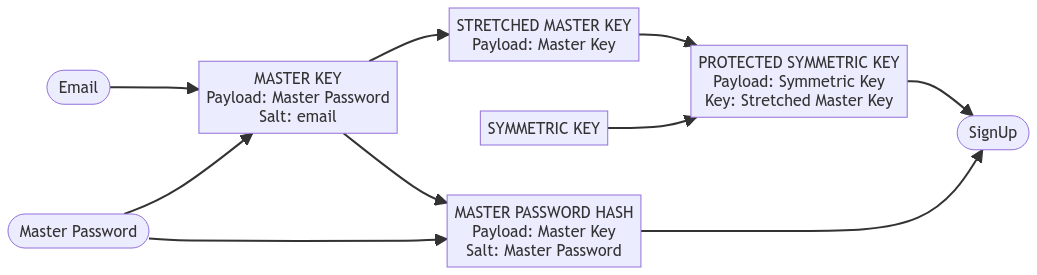
\includegraphics[width=1.0\textwidth]{figures/infoEncription}
        %\caption*{a nice plot}
    \end{figure}
Il sistema di cifratura opera interamente lato client e tutti i dati trasmessi da e verso i server sono crittografati end-to-end, anche qualora l'utente effettui l'accesso da un nuovo dispositivo. In questo modo, anche ipotizzando una compromissione dei server, i dati rimarranno comunque riservati. La sicurezza degli stessi è quindi demandata alla robustezza della password scelta dall'utente in fase di creazione dell'account (la quale richiede determinati requisiti di complessità).

È possibile schematizzare la fase di registrazione nei seguenti punti:
\begin{itemize}
    \item Viene generata la \textit{Master Key} utilizzando la \textit{Master Password} come payload e l'indirizzo email come salt;
    \item Viene creata la \textit{Stretched Master Key} utilizzando la \textit{Master Key} come payload;
    \item Viene generata la \textit{Simmetric Key} a 512-bit utilizzando una funzione randomica sicura. Questa è la chiave di cifratura dei dati dell'utente;
    \item Viene creata la \textit{Protected Symmetric Key} cifrando la \textit{Simmetric Key} mediante la \textit{Stretched Master Key} e un vettore di inizializzazione casuale. Questa chiave verrà condivisa al server e ai dispositivi in cui l'utente effettua l'accesso.
\end{itemize}

Poiché la \textit{Master Password} deve essere mantenuta segreta, in fase di registrazione viene inviato al backend l'hash della stessa (oltre che la \textit{Protected Symmetric Key} chiamata nell'uso \texttt{Magic Key}) e questo provvederà a conservare il suo ulteriore hash insieme ad un salt. L'hash della \textit{Master Password}, generato dal client, può essere quindi considerato come il criterio di identificazione dell'utente, mantenendo al contempo la riservatezza dei suoi dati cifrati.

A seguito di un accesso andato a buon fine il client scarica la \textit{Protected Symmetric Key}, e, tramite un procedimento analogo a quello della registrazione, una volta inseriti indirizzo email e \textit{Master Password}, decifra la \textit{Simmetric Key} tramite la \textit{Stretched Master Key} (nuovamente calcolata) con cui è possibile decifrare la cassaforte.

La procedura di cambio \textit{Master Password}, anch'essa effettuata in locale, prevede una nuova cifratura della stessa \textit{Simmetric Key} (essendo cambiato il payload iniziale) e la condivisione al server della nuova \textit{Protected Symmetric Key}.

\chapter{Interfacce}

WizardGuard è usufruibile in tema chiaro/scuro e multilingua (attualmente italiano/inglese).

\section{Form di registrazione}
    \begin{figure}[H]
        \centering
        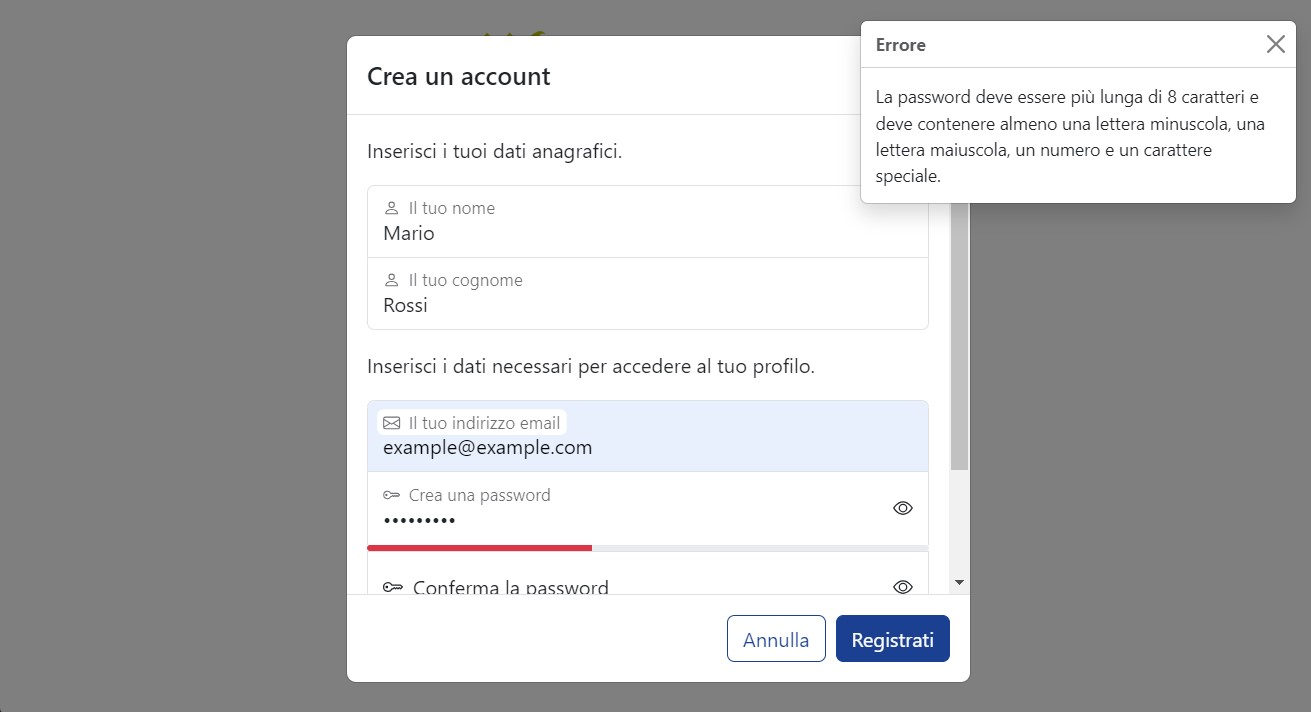
\includegraphics[width=1.0\textwidth]{figures/interfaces/signup}
        %\caption*{a nice plot}
    \end{figure}

\section{Form di accesso}
    \begin{figure}[H]
        \centering
        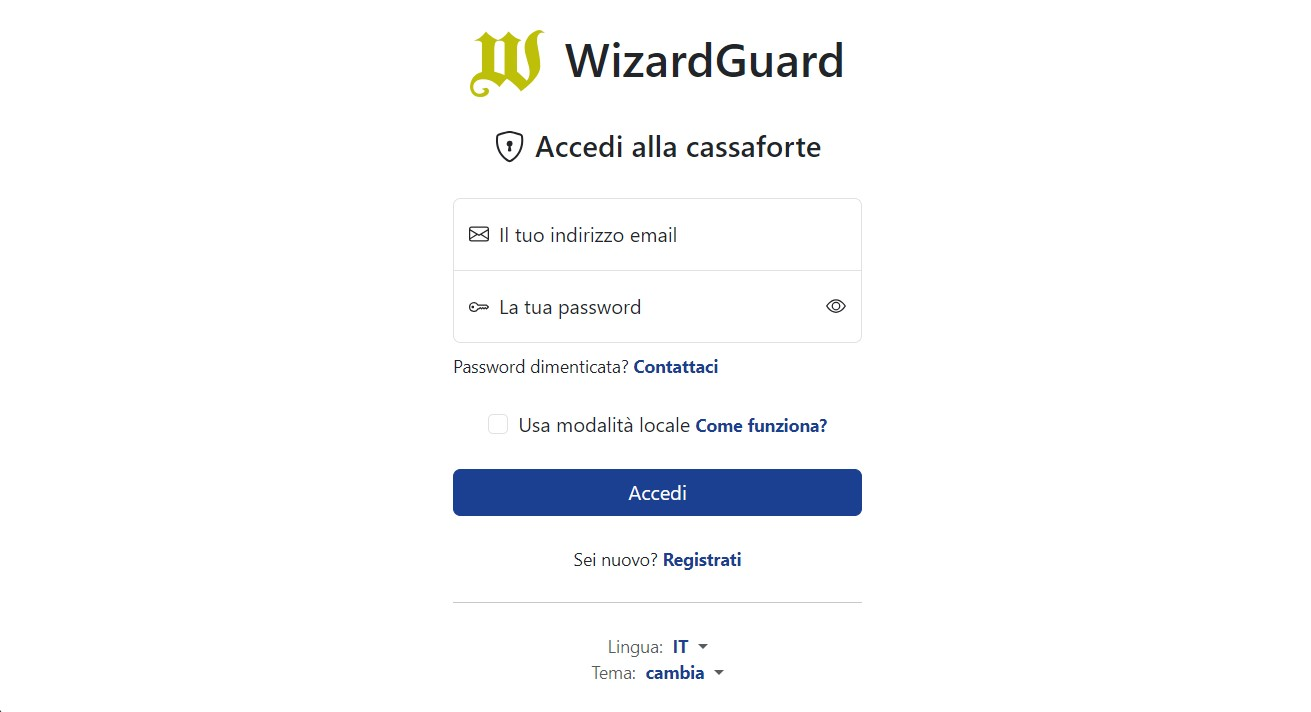
\includegraphics[width=1.0\textwidth]{figures/interfaces/signin}
        %\caption*{a nice plot}
    \end{figure}
    
\section{Cassaforte bloccata}
\begin{figure}[H]
        \centering
        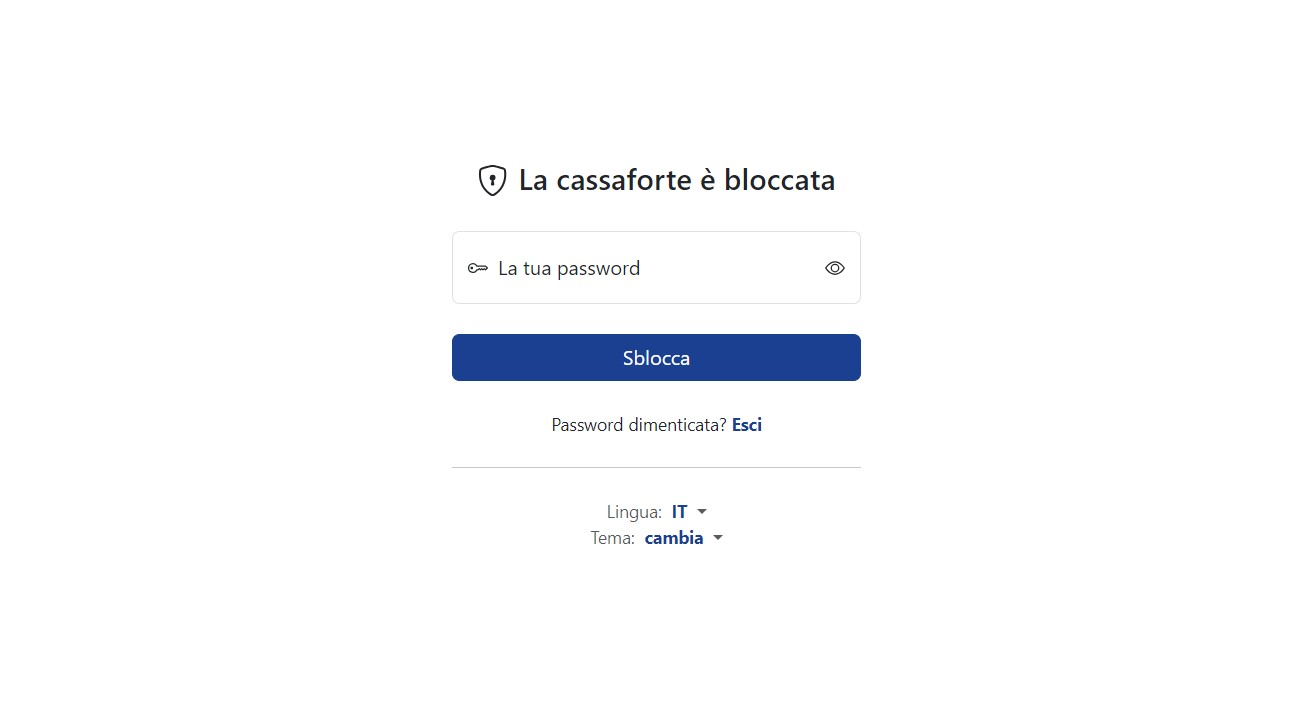
\includegraphics[width=1.0\textwidth]{figures/interfaces/unlock}
        %\caption*{a nice plot}
    \end{figure}
\section{Cassaforte}
\begin{figure}[H]
        \centering
        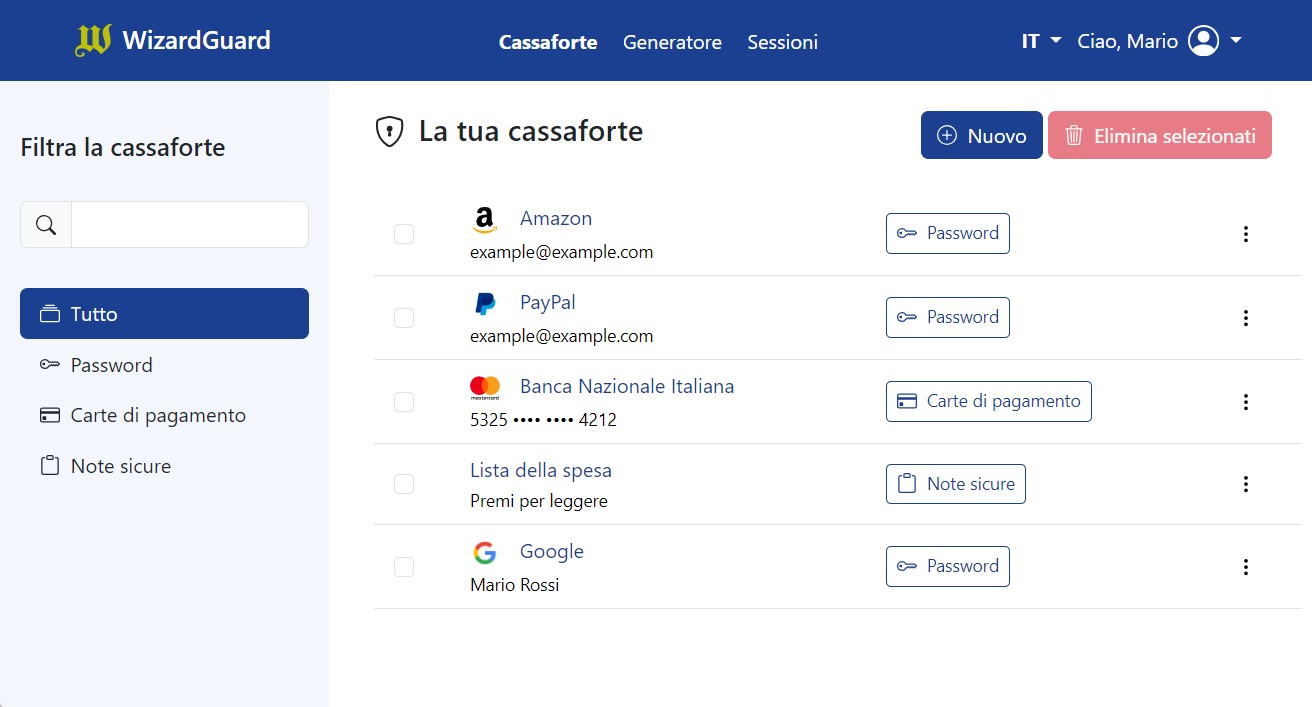
\includegraphics[width=1.0\textwidth]{figures/interfaces/vault}
        %\caption*{a nice plot}
    \end{figure}
\section{Elemento della cassaforte}
\begin{figure}[H]
        \centering
        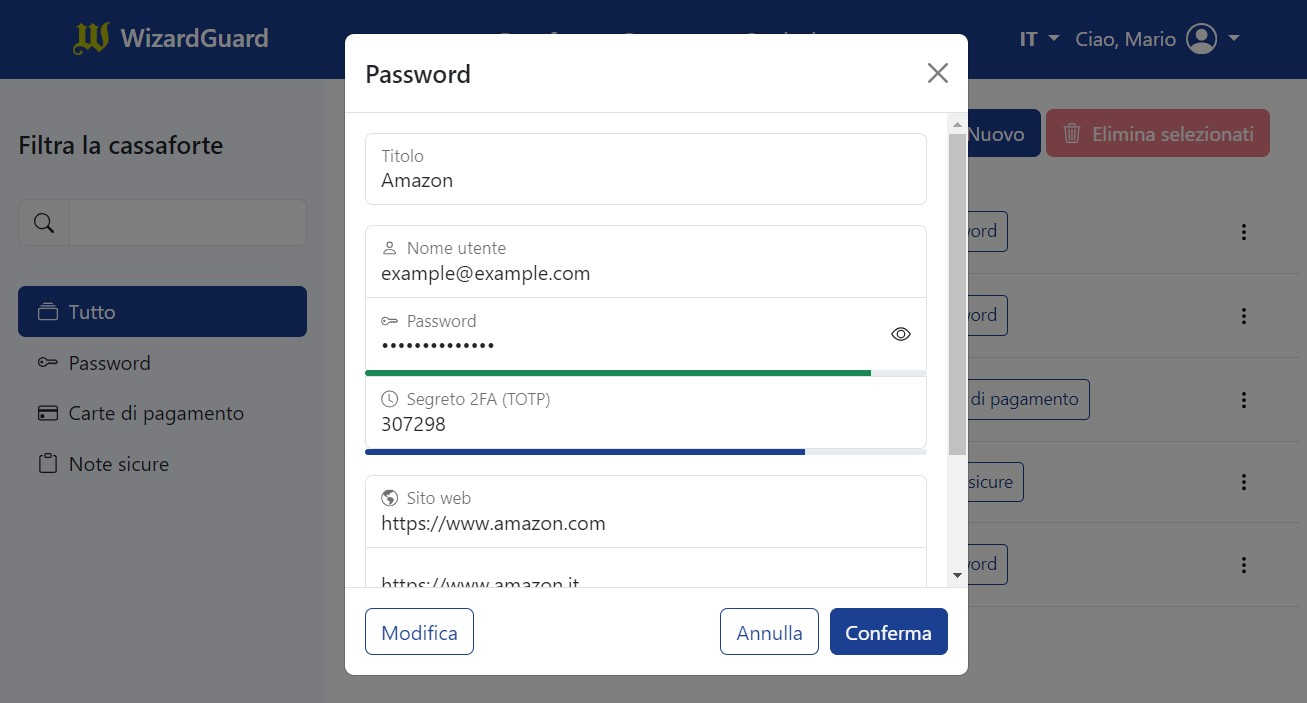
\includegraphics[width=1.0\textwidth]{figures/interfaces/element}
        %\caption*{a nice plot}
    \end{figure}
\section{Sessioni}
\begin{figure}[H]
        \centering
        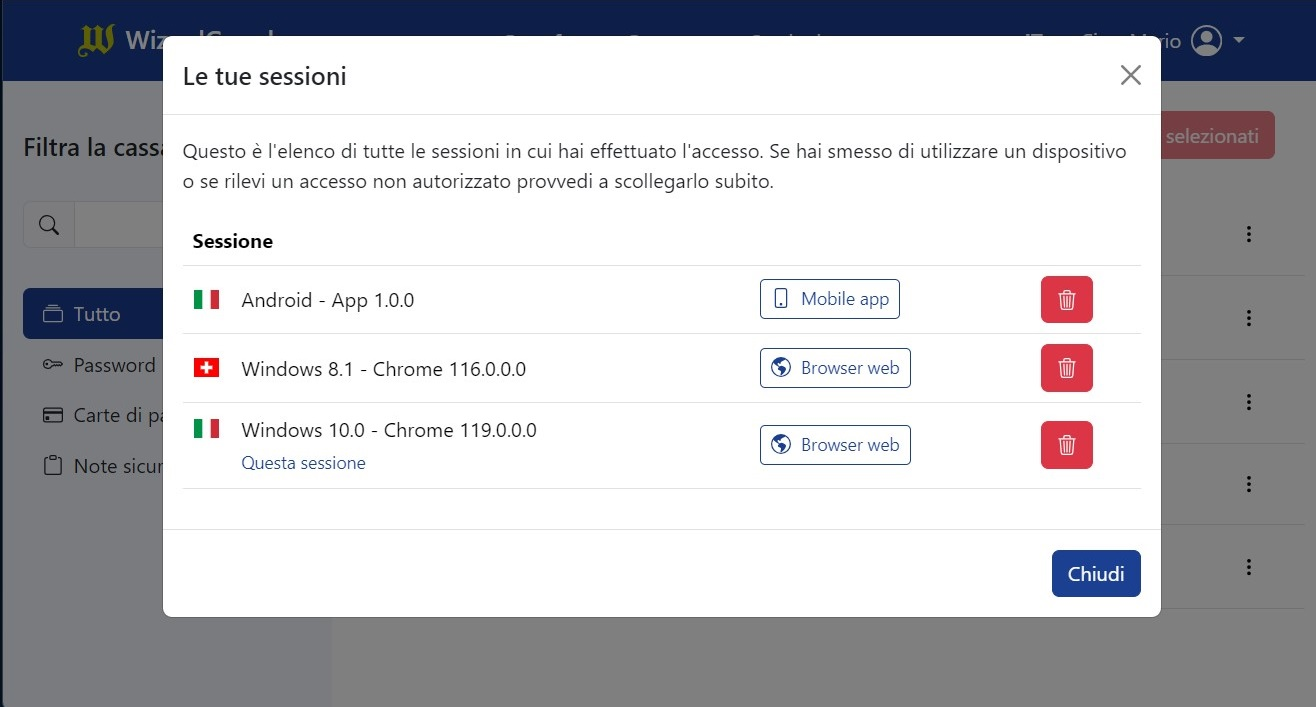
\includegraphics[width=1.0\textwidth]{figures/interfaces/sessions}
        %\caption*{a nice plot}
    \end{figure}
\section{Generatore di password}
\begin{figure}[H]
        \centering
        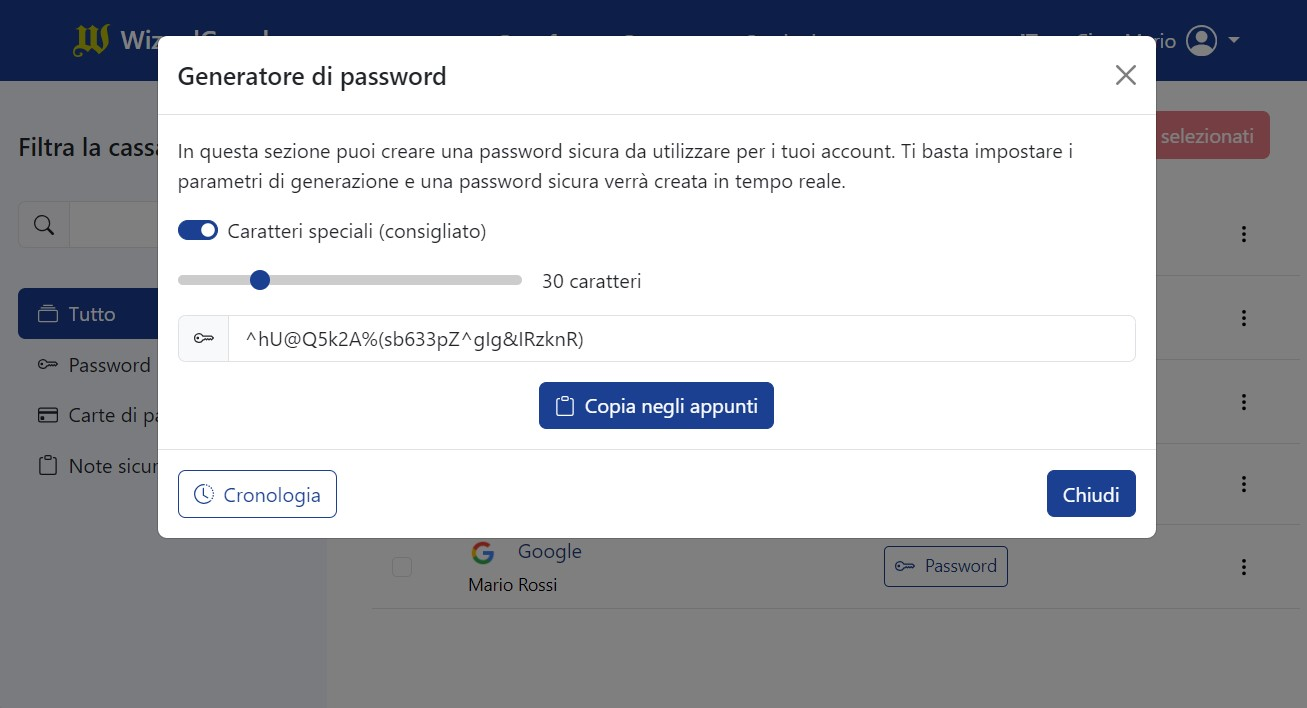
\includegraphics[width=1.0\textwidth]{figures/interfaces/passwordGenerator}
        %\caption*{a nice plot}
    \end{figure}
\section{Profilo utente}
\begin{figure}[H]
        \centering
        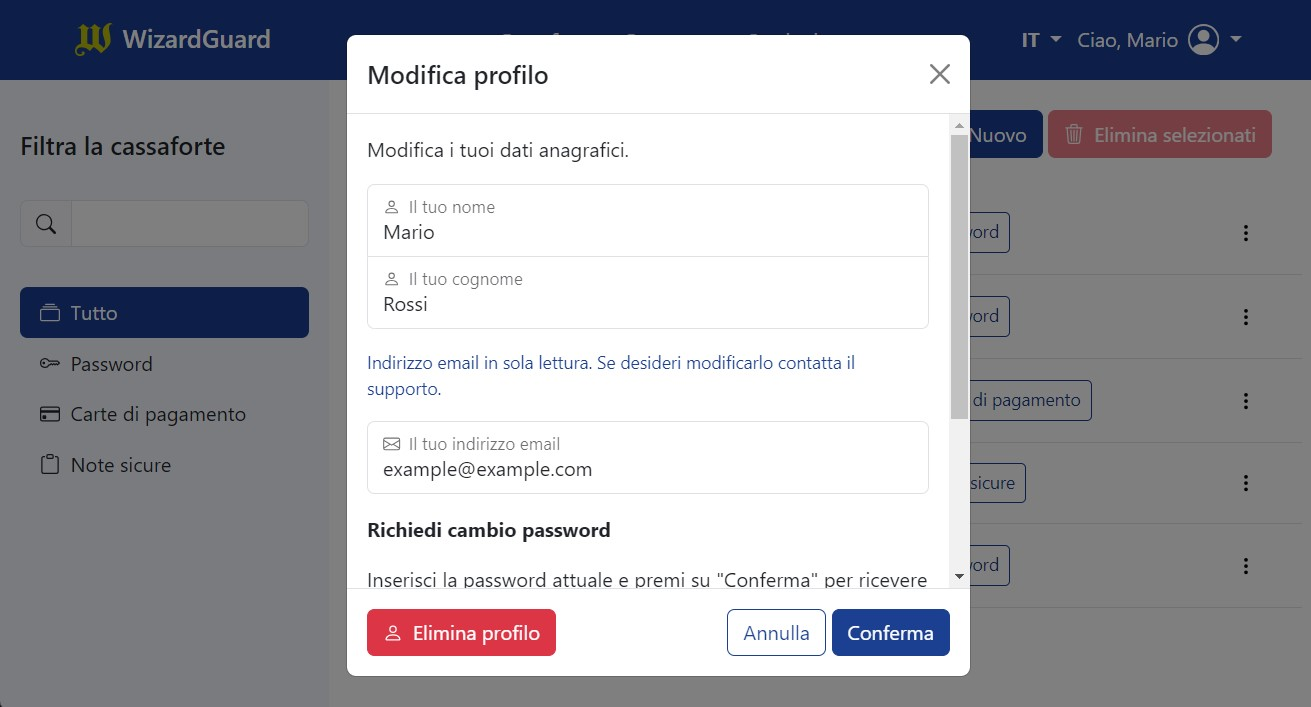
\includegraphics[width=1.0\textwidth]{figures/interfaces/profile}
        %\caption*{a nice plot}
    \end{figure}
\section{Template email di benvenuto}
\begin{figure}[H]
        \centering
        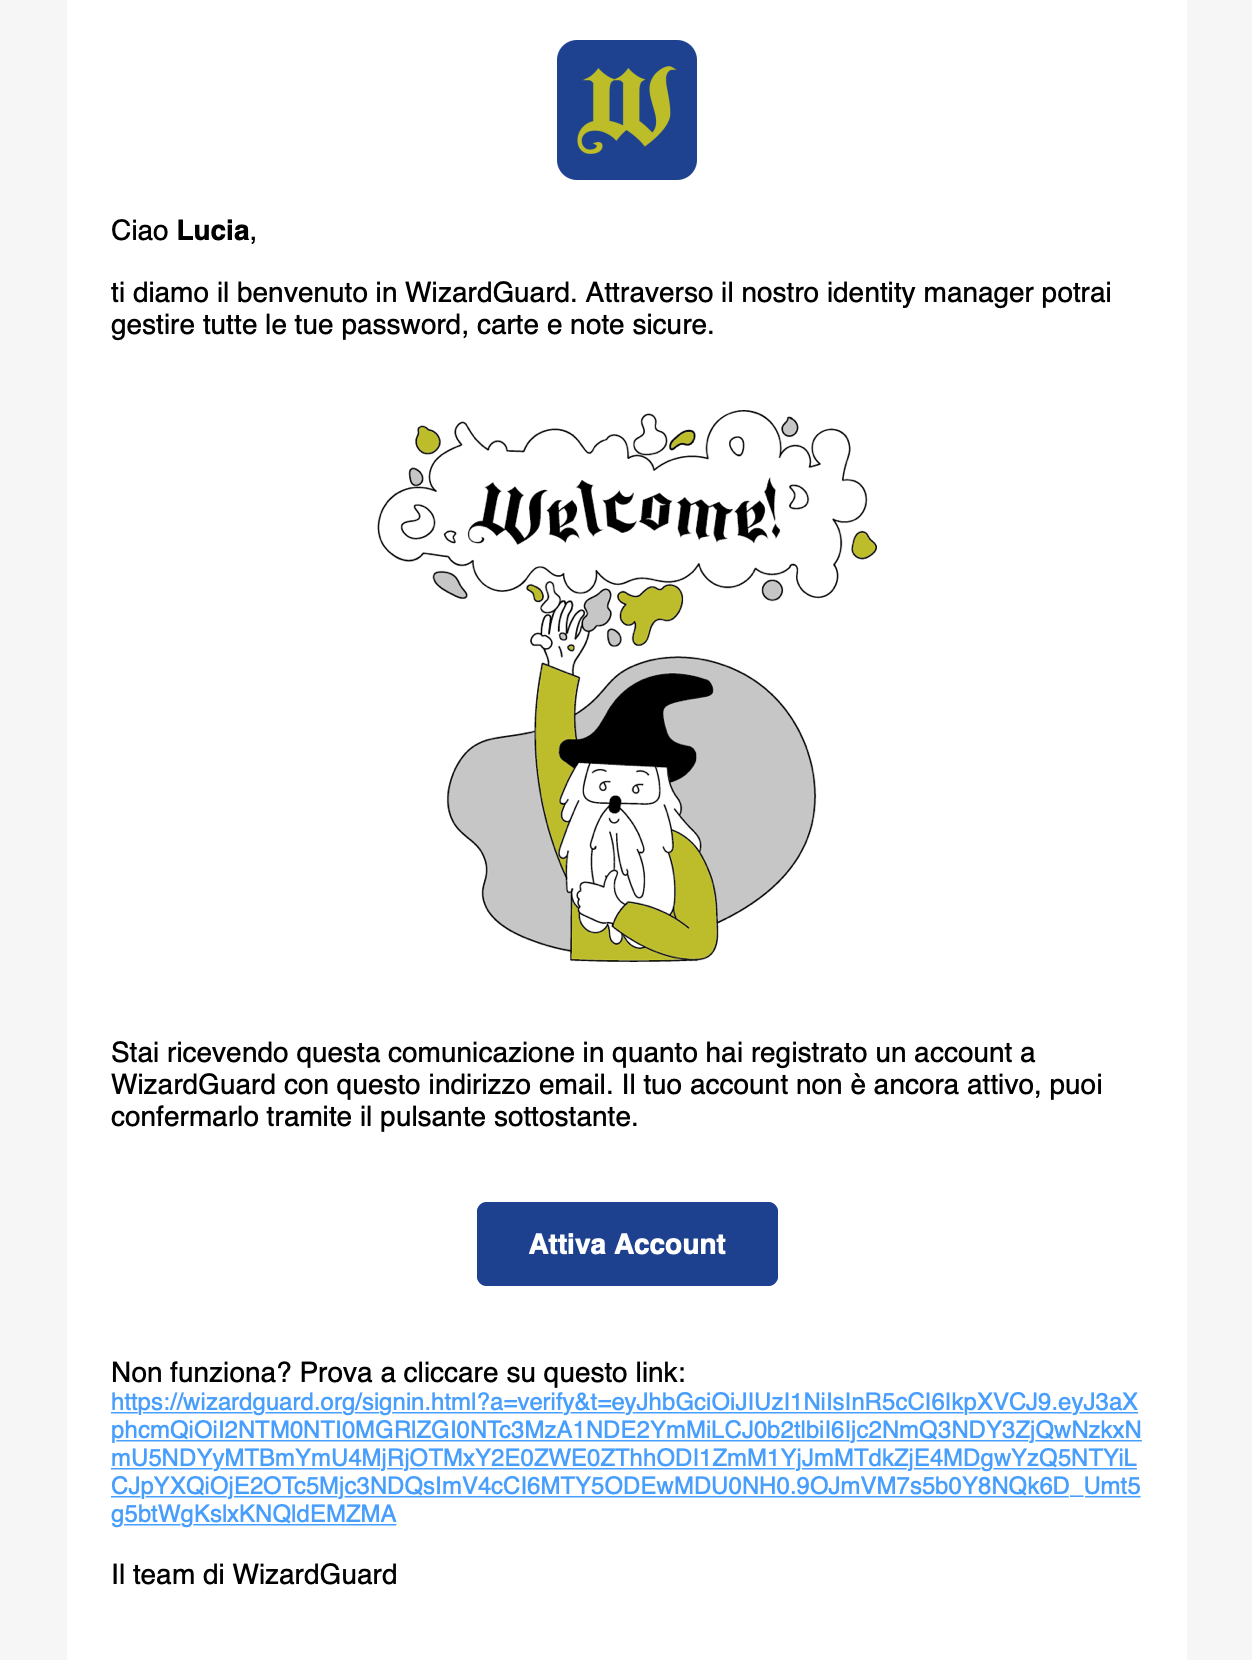
\includegraphics[width=0.47\textwidth]{figures/interfaces/welcomeEmail}
        %\caption*{a nice plot}
    \end{figure}
\section{Template email di eliminazione utente}
\begin{figure}[H]
        \centering
        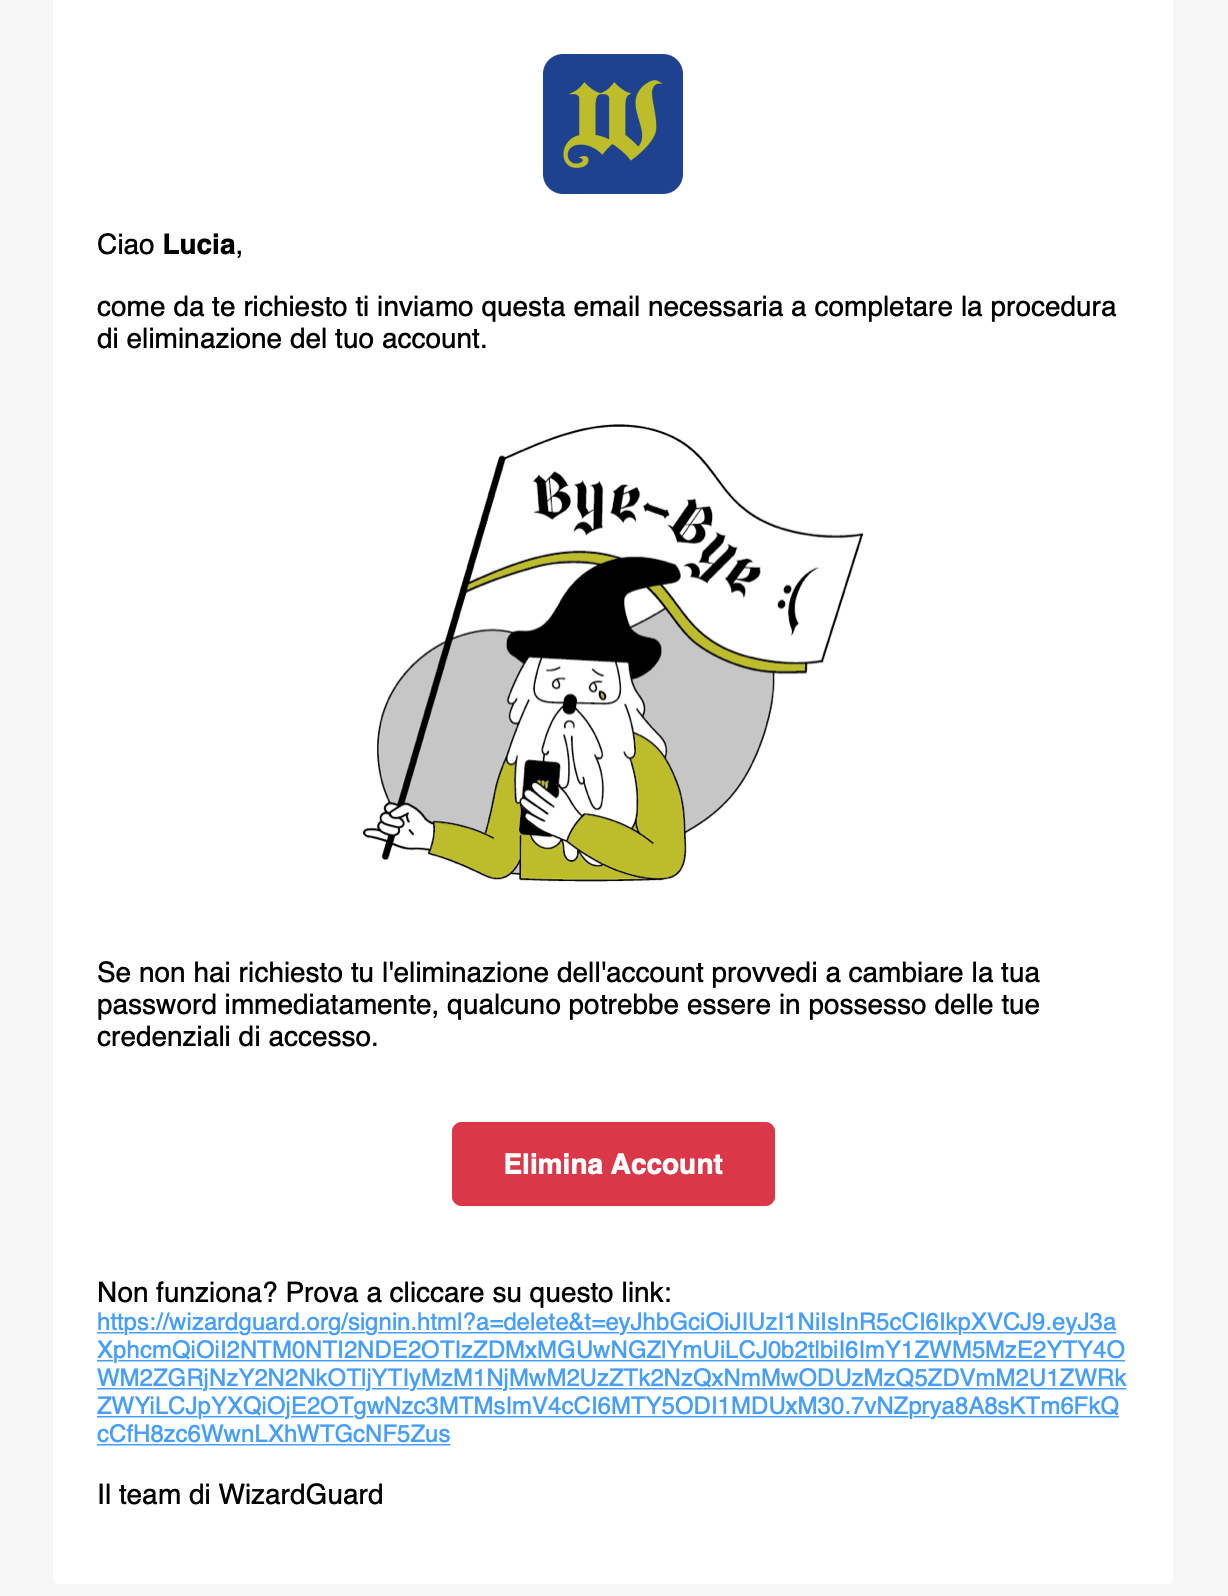
\includegraphics[width=0.47\textwidth]{figures/interfaces/goodbyeEmail}
        %\caption*{a nice plot}
    \end{figure}
\chapter{Architettura}
\section{Diagramma dell'ordine gerarchico delle risorse}
Si riportano le funzionalità di frontend accessibili dall'utente e le loro transazioni con le relative chiamate API a backend.

\begin{figure}[H]
        \centering
        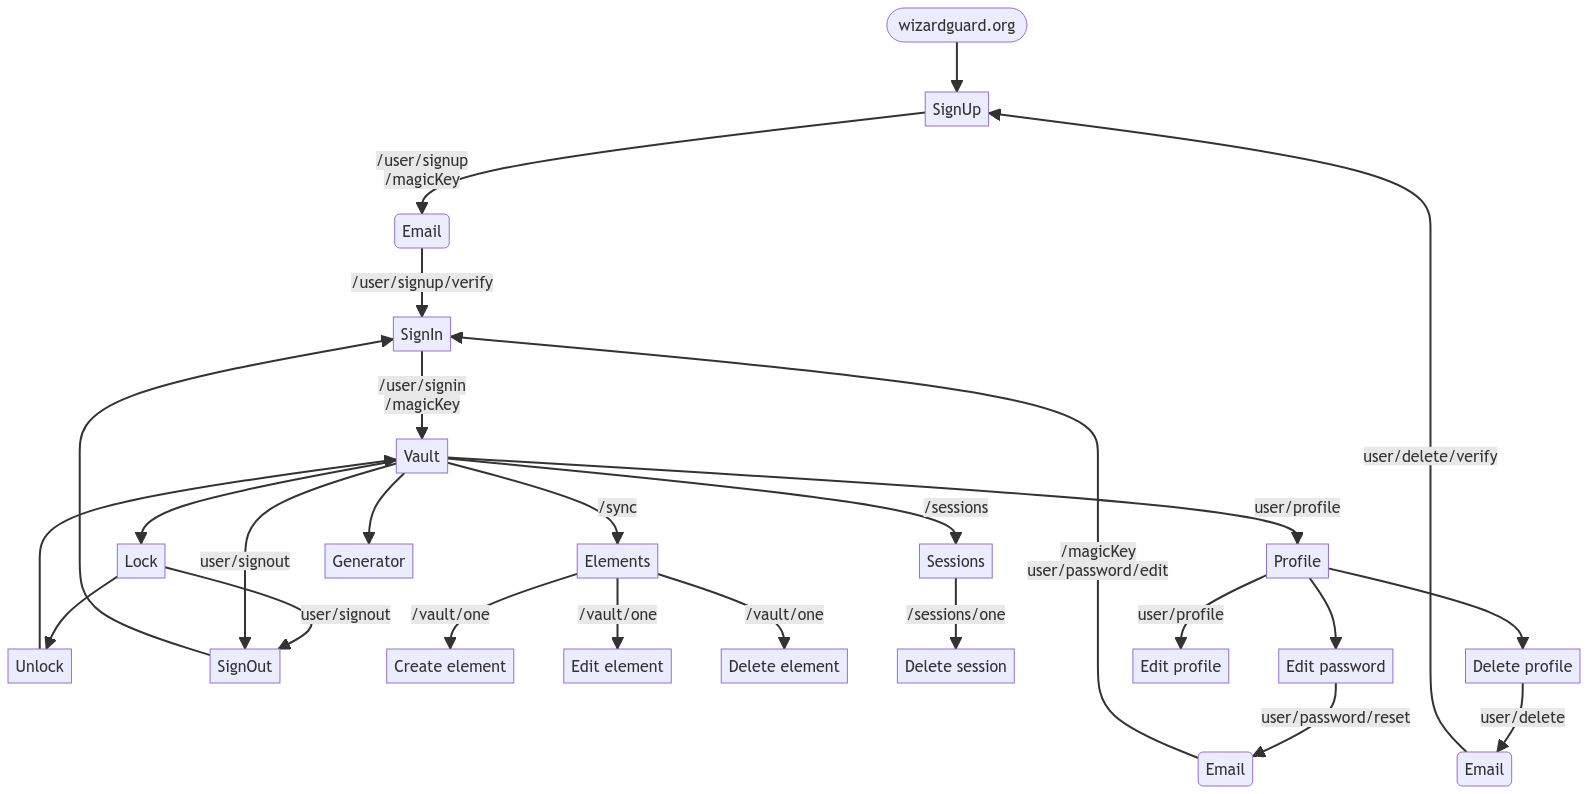
\includegraphics[width=1.0\textwidth]{figures/architectures/hierarchicalOrder}
        %\caption*{a nice plot}
    \end{figure}
\section{Diagramma di flusso}
\subsection{Backend}
\begin{figure}[H]
        \centering
        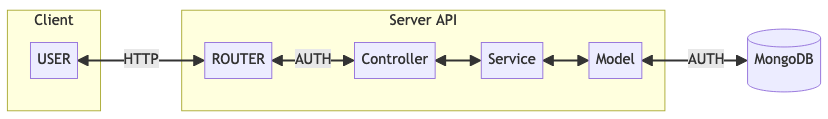
\includegraphics[width=1.0\textwidth]{figures/architectures/apiFlowChart}
        %\caption*{a nice plot}
    \end{figure}
Le richieste al server api arrivano tramite protocollo HTTP Sicuro e vengono smistate dal Router che richiama la funzione dedicata. 


Tutti gli endpoint forniscono dati tramite JSON nel body della richiesta. In base alla chiamata effettuata vengono fatti i controlli preliminari previsti (autenticazione e/o validazione dati inviati). 
\begin{itemize}
    \item Il \textbf{Controller} gestisce la richiesta e si occupa di comporre la risposta;
    \item Al \textbf{Service} vengono demandate le elaborazioni riferite alla chiamata invocata;
    \item Il \textbf{Model} gestisce le relazioni dirette con la base di dati.
\end{itemize}
\section{Descrizione delle risorse}

Per la struttura delle risposte fornite dalle API di backend si è scelto di seguire le specifiche JSend\cite{jsend}. Tutte le risposte rispettano la seguente struttura:

\begin{minted}{text}
{
    status: "success | fail | error",
    data: {} | message: "..."
}
\end{minted}

In particolare il campo \texttt{data} viene indicato solo con il campo \texttt{status} valorizzato come:
\begin{itemize}
    \item \textbf{success}: contiene i dati inviati (\texttt{PUT}/\texttt{POST}) o richiesti (\texttt{GET}), altrimenti \texttt{null};
    \item \textbf{fail}: contiene un array di oggetti ognuno dei quali ha come chiave l'elemento della richiesta coinvolto dal fail e come valore, un messaggio in inglese in merito.
    \begin{minted}{json}
{
    "name.firstName": "User first name is required"
}
    \end{minted}
\end{itemize}
Nel caso \texttt{status: "error"}, viene proposto il campo \texttt{message}, valorizzato con un messaggio di errore, nella lingua associata all'header della richiesta o nel caso la lingua non fosse suppotata, in inglese.
\\\\
Vengono di seguito elencati nel dettaglio tutti gli endpoint delle API di backend.
\subsection*{auth}
\begin{center}
\setlength\extrarowheight{4pt}
\begin{tabularx}{\textwidth}{|X|l|X|}
\hline
  \textbf{Endpoint} & \textbf{Auth} & \textbf{Descrizione}\\
\hline
\texttt{POST auth/refreshTokens}  &  \hspace{0.2cm}\faIcon{lock-open}  & Generazione nuovi auth token e modifica sessione \\
\hline
\end{tabularx}
\end{center}

\subsection*{user}
\begin{center}
\setlength\extrarowheight{4pt}
\begin{tabularx}{\textwidth}{|X|l|X|}
\hline
  \textbf{Endpoint} & \textbf{Auth} & \textbf{Descrizione}\\
\hline
\texttt{POST user/signup}  &  \hspace{0.2cm}\faIcon{lock-open}  & Registrazione nuovo utente \\
\hline
\texttt{POST user/signup/verify}  &  \hspace{0.2cm}\faIcon{lock-open}  & Verifica e attivazione nuovo utente \\
\hline
\texttt{POST user/signin}  &  \hspace{0.2cm}\faIcon{lock-open}  & Accesso utente \\
\hline
\texttt{POST user/signout}  &  \hspace{0.2cm}\faIcon{lock}  & Uscita utente ed eliminazione sessione \\
\hline
\texttt{GET user/profile}  &  \hspace{0.2cm}\faIcon{lock}  & Fornisce i dati utente (nome e email) \\
\hline
\texttt{PUT user/profile}  &  \hspace{0.2cm}\faIcon{lock}  & Modifica i dati utente (nome e email) \\
\hline
\texttt{POST user/delete}  &  \hspace{0.2cm}\faIcon{lock}  & Invio email per eliminazione account \\
\hline
\texttt{DELETE user/delete/verify}  &  \hspace{0.2cm}\faIcon{lock-open}  & Verifica ed eliminazione utente \\
\hline
\texttt{POST user/password/reset}  &  \hspace{0.2cm}\faIcon{lock}  & Invio email per cambio password\\
\hline
\texttt{PUT user/password/edit}  &  \hspace{0.2cm}\faIcon{lock-open}  & Cambio password \\
\hline
\end{tabularx}
\end{center}

\subsection*{sessions}
\begin{center}
\setlength\extrarowheight{4pt}
\begin{tabularx}{\textwidth}{|X|l|X|}
\hline
  \textbf{Endpoint} & \textbf{Auth} & \textbf{Descrizione}\\
\hline
\texttt{GET sessions}  &  \hspace{0.2cm}\faIcon{lock}  & Fornisce l'elenco delle sessioni (indicando quella corrente) \\
\hline
\texttt{DELETE sessions}  &  \hspace{0.2cm}\faIcon{lock}  & Elimina le sessioni (opzione elimina tutte o eccetto sessione corrente) \\
\hline
\texttt{DELETE sessions/one}  &  \hspace{0.2cm}\faIcon{lock}  & Elimina la sessione indicata \\
\hline
\end{tabularx}
\end{center}

\subsection*{magicKey}
\begin{center}
\setlength\extrarowheight{4pt}
\begin{tabularx}{\textwidth}{|X|l|X|}
\hline
  \textbf{Endpoint} & \textbf{Auth} & \textbf{Descrizione}\\
\hline
\texttt{POST magicKey}  &  \hspace{0.2cm}\faIcon{lock}  & Aggiunge/modifica la magic key \\
\hline
\texttt{GET magicKey}  &  \hspace{0.2cm}\faIcon{lock}  & Fornisce la magic key \\
\hline
\end{tabularx}
\end{center}

\subsection*{vault}
\begin{center}
\setlength\extrarowheight{4pt}
\begin{tabularx}{\textwidth}{|X|l|X|}
\hline
  \textbf{Endpoint} & \textbf{Auth} & \textbf{Descrizione}\\
\hline
\texttt{GET vault}  &  \hspace{0.2cm}\faIcon{lock}  & Fornisce la cassaforte utente \\
\hline
\texttt{POST vault}  &  \hspace{0.2cm}\faIcon{lock}  & Aggiunge elementi alla cassaforte utente \\
\hline
\texttt{PUT vault}  &  \hspace{0.2cm}\faIcon{lock}  & Modifica elementi della cassaforte utente \\
\hline
\texttt{DELETE vault}  &  \hspace{0.2cm}\faIcon{lock}  & Elimina la cassaforte utente \\
\hline
\texttt{POST vault/one}  &  \hspace{0.2cm}\faIcon{lock}  & Aggiunge un elemento alla cassaforte utente \\
\hline
\texttt{PUT vault/one}  &  \hspace{0.2cm}\faIcon{lock}  & Modifica un elemento della cassaforte utente \\
\hline
\texttt{DELETE vault/one}  &  \hspace{0.2cm}\faIcon{lock}  & Elimina un elemento della cassaforte utente \\
\hline
\end{tabularx}
\end{center}

\section{Autenticazione}
L'accesso agli endpoint delle API di backend è gestito mediante autenticazione tramite JWT\cite{jwt}. Alcuni endpoint non autenticati (\texttt{user/signin}, \texttt{user/signup}, \texttt{auth/refreshTokens}) permettono di ricevere nella risposta \textit{Access Token} e \textit{Refresh Token}, da utilizzare per le chiamate autenticate. I token contengono dei dati crittografati, utili per le richieste, e sono soggetti ad una scadenza (10 minuti per l\/'\textit{Access Token} e 14 giorni per il \textit{Refresh Token}).


Una volta ricevuti i token, il client li salva e utilizza l'\textit{Access Token} (inserendolo opportunamente nell'header della richiesta) per autenticarsi. Una volta che l'\textit{Access Token} scade, le richieste saranno rifiutate perchè non autorizzate, a questo punto tramite un endpoint specifico (\texttt{auth/refreshTokens}) sarà possibile, fornendo il \textit{Refresh Token}, ricevere una nuova coppia di token. 


Per tenere traccia delle sessioni attive, ad un nuovo accesso dell'utente viene creata una nuova sessione utente sul database, a cui è associato il \textit{Refresh Token}. La verifica dei token, oltre che crittografica e di validità di tempo, è di consistenza vagliando la lista delle sessioni utente sul database.

\section{Database e modelli}
La struttura del database è stata modellata realizzando una singola collection riferita all'utente e alle sue attività. In particolare oltre ai dettagli dell'utente sono archiviate le sessioni personali attive e le stringhe criptate relative alla sua cassaforte. Di seguito viene proposto per esteso, il modello della collection, così come viene validato dal database.
\begin{minted}{json}
"$jsonSchema": {
  "bsonType": "object",
  "required": ["user", "magicKey", "sessions", "vault"],
  "properties": {
    "user": {
      "bsonType": "object",
      "required": ["name", "email", "masterPassword", "isActive", "validationToken", "isEnabled", "creationTimestamp"],
      "properties": {
        "name": {
          "bsonType": "object",
          "required": ["firstName", "lastName"],
          "properties": {
            "firstName": { "bsonType": "string" },
            "lastName": { "bsonType": "string"}
          }
        },
        "email": {
          "bsonType": "string"
        },
        "masterPassword": {
          "bsonType": "object",
          "required": ["value", "salt"],
          "properties": {
            "value": { "bsonType": "string" },
            "salt": { "bsonType": "string" }
          }
        },
        "isActive": { "bsonType": "bool" },
        "validationToken": { "bsonType": "string" },
        "isEnabled": { "bsonType": "bool" },
        "creationTimestamp": { "bsonType": "date" }
      }
    },
    "magicKey": { "bsonType": "string" },
    "sessions": {
      "bsonType": "array",
      "items": {
        "bsonType": "object",
        "required": ["id", "location", "userAgent", "refreshToken"],
        "properties": {
          "id": { "bsonType": "objectId" },
          "location": {
            "bsonType": "string",
            "minLength": 2,
            "maxLength": 2
          },
          "userAgent": {
            "bsonType": "object",
            "required": ["device", "client", "type"],
            "properties": {
              "device": { "bsonType": "string" },
              "client": { "bsonType": "string" },
              "type": { "enum": ["web", "mobile", "unknown"] }
            }
          },
          "refreshToken": {
            "bsonType": "object",
            "required": ["value", "expiration"],
            "properties": {
              "value": { "bsonType": "string" },
              "expiration": { "bsonType": "date" }
            }
          }
        }
      }
    },
    "vault": {
      "bsonType": "array",
      "items": {
        "bsonType": "object",
        "required": ["id", "value", "updatedAt"],
        "properties": {
          "id": { "bsonType": "objectId" },
          "value": { "bsonType": "string" },
          "updatedAt": { "bsonType": "string" }
        }
      }
    }
  }
}
\end{minted}

\section{Diagramma di flusso app mobile}
Attraverso il framework Apache Cordova è stato possibile utilizzare l'interfaccia grafica e la logica principale dell'applicazione precedentemente sviluppata, ottimizzando i tempi di sviluppo e uniformando l'usabilità per a livello utente.

Cordova permette inoltre integrazioni con il sistema operativo tramite plugin appositamente sviluppati. Tali plugin non sono stati tuttavia utilizzati in quanto non risulta necessario accedere a specifiche funzioni di sistema.

Per la specifica versione Android sono stati definiti icona e splash screen nel file config.xml, è stata inoltre creata la classe \texttt{WizardGuardAutofillService.java}, registrata come servizio in AndroidManifest.xml, demandata ad utilizzare l'API di sistema di AutoFill necessaria a identificare i campi password e a proporre l'apertura dell'app in tali contesti.

\begin{figure}[H]
        \centering
        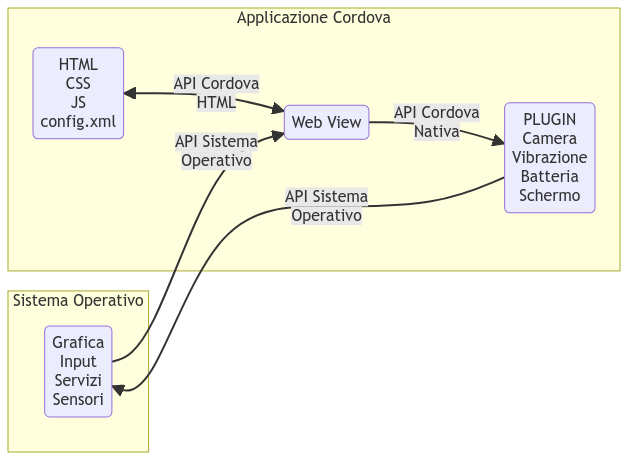
\includegraphics[width=0.7\textwidth]{figures/architectures/cordova}
        %\caption*{a nice plot}
    \end{figure}
\chapter{Codice}
\section{Struttura del progetto}
Di seguito i riportano le strutture dei due repository git di produzione di frontend e backen.
\subsection{Frontend}
Nella cartella principale del progetto sono presenti:
\begin{itemize}
    \item cartella \textbf{css}: contenente i fogli di stile;
    \item cartella \textbf{img}: contenente le immagini statiche;
    \item cartella \textbf{js}: contenente le logiche applicative javascript;
    \item \textbf{cordova.js}: file popolato da Cordova alla compilazione dell'applicazione;
    \item \textbf{index.html}: file di redirect alla signin;
    \item \textbf{signin.html}: pagina di registrazione ed accesso utente;
    \item \textbf{unlock.html}: pagina di blocco/sblocco della cassaforte;
    \item \textbf{vault.html}: pagina della cassaforte (autenticata).
\end{itemize}
\subsection{Backend}
Nella cartella principale del progetto sono presenti:
\begin{itemize}
    \item cartella \textbf{src}: contenente tutti i file Node.js del backend;
    \item cartella \textbf{tests}: cartella vuota per l'implementazione futura degli unit test del backend;
    \item \textbf{package.json}: file di configurazione del progetto NPM, com indicate le dipendenze di pacchetti utilizzate.
\end{itemize}
Si precisa ora la struttura della cartella \textbf{src}:
\begin{itemize}
    \item \textbf{app.js}: file principale dell'applicazione dove:
        \begin{itemize}
            \item viene eseguita la connessione al dabatase MongoDB;
            \item viene creato e configurato il server Express;
            \item vengono specificati i router degli enpoint delle api;
            \item viene gestita la risposta in caso di error, fail o eccezioni;
            \item viene avviato il server, in ascolto sulla porta 3434 (modificata da Render a 1000).
        \end{itemize}
    \item \textbf{config.js}: file javascript contentente alcune variabili di impostazione;
    \item cartella \textbf{controllers};
    \item cartella \textbf{services};
    \item cartella \textbf{routes};
    \item cartella \textbf{data}: contenente alcuni file statici di configurazioone (codici di errore e template mail multilingua).
\end{itemize}
Nel repository di produzione del backend non è presente il file \textbf{.env}, in quanto le variabili di ambiente utilizzate (credenziali database e chiavi di cifratura token) sono indicate direttamente nella configurazione di progetto di Render.
\section{Backend}
Si riportano le funzioni di verifica dei token di autenticazione, in particolare la funzione \texttt{authenticateToken} viene chiamata prima dell'esecuzione del codice specifico dell'endpoint autenticato chiamato, e dell'eventuale validazione del body della richiesta. La verifica, come spiegato in precedenza, viene effettuata sia tramite il controller dei token JWT, quindi verificando la corretta decifratura dei dati contenuti nel token e la sua validità temporale, che verificando l'esistenza della sessione corrispondente tra quelle associate all'utente nel database.
La funzione \texttt{verifyControlToken} riguarda invece la verifica di un token artificiale, creato sempre tramite JWT, con una chiave di cifratura dedicata, utilizzato come paramentro nel link inviato all'utente via mail, nelle operazioni di verifica utenza, cambio password ed eliminazione utenza.
\begin{minted}{javascript}
const TokenController = require("./token");
const Exception = require("../exception");
const SessionModel = require("../../models/session");
const UserModel = require("../../models/user");
const UserController = require("../../controllers/user");

exports.authenticateToken = async (req, res, next) => {
  const authHeader = req.headers["authorization"];
  if (typeof authHeader !== 'undefined') {
    const token = authHeader.split(" ")[1];
    if (token !== null) {
      try {
        const tokenData = TokenController.verifyAccessToken(token);
        if (!(await SessionModel.getRefreshToken(tokenData.wizard, tokenData.session)))
          return next(new Exception(106));
        req.auth = tokenData;
        return next();
      } catch (err) {
        next(new Exception(106));
      }
    }
  }
  next(new Exception(106));
}

exports.verifyControlToken = async (controlToken) => {
  const tokenData = TokenController.verifyControlToken(controlToken);
  if (!tokenData)
    return false;
  const verifyFlag = await UserModel.verifyUserTokenById(tokenData.wizard, tokenData.token);
  const updateFlag = await UserController.updateUserToken(tokenData.wizard);
  return verifyFlag && updateFlag ? tokenData.wizard : false;
}
\end{minted}
Di seguito vengono mostrate due funzioni associate a due differenti endpoint, il primo \texttt{user/signin} (non autenticato) permette di effettuare l'accesso, inserendo i dati di autenticazione utente nel body della richiesta. La risposta restituisce il nome dell'utente e i token necessari alle successive chiamate autenticate. Nella funzione, dopo aver verificato i dati di accesso dell'utente, viene creata una nuova sessione associata al Refresh Token generato e viene effettuato un controllo sulla localizzazione dell'ip della richiesta utente e, nel caso sia riferito ad una nazione inedita per l'utente, lo stesso viene avvisato con una email.
\begin{minted}{javascript}
router.post('/signin', userSignInDataValidateChain, async (req, res, next) => {
  try {
    if (!(fail = validationResult(req)).isEmpty())
      return next(new Fail(fail.array()));
    const user = await UserController.signin(req.body.email, req.body.password);
    if (!user)
      return next(new Exception(107));
    if (!user.isActive)
      return next(new Exception(115));
    const sessionId = SessionController.generateSessionId();
    const tokens = AuthController.generateTokens(user.wizard, req.body.email, sessionId);
    await SessionController.pushSession(user.wizard, sessionId, req.ip, req.useragent, tokens.refreshToken);
    const data = ResponseController.concatTwo({
      name: user.name
    }, tokens);
    response.setSuccess(data);
    const location = getLocationByIp(req.ip);
    if (await SessionModel.isNewCountry(user.wizard, location.iso)) {
      lang = req.acceptsLanguages(acceptedLanguages);
      await EmailController.sendNewLocationEmail(user.name, req.body.email, lang, user.wizard, user.validationToken, location.ext);
    }
    res.status(response.getHttpCode()).json(response.getResponse());
  } catch (error) {
    next(error);
  }
});
\end{minted}
Infine si mostrano due funzioni del \texttt{SessionModel}, in particolare la prima permette di inserire una nuova sessione sul database, mentre la seconda elimina tutte le sessioni utente presenti (con l'eventualità di mantenere quella corrente specificandone l'id come paramentro).
\begin{minted}{javascript}
const WizardModel = require('./wizard');

exports.pushSession = async (wizard, session, location, userAgent, refreshToken, expiration) => {
  const sessionData = {
    id: session,
    location: location,
    userAgent: userAgent,
    refreshToken: {
      value: refreshToken,
      expiration: expiration
    }
  };
  await WizardModel.updateOne({
    "_id": wizard
  }, {
    $push: {
      "sessions": sessionData
    }
  });
};

...

exports.clearSessions = async (wizard, id = undefined) => {
  if (id === undefined)
    return await WizardModel.updateOne({
      "_id": wizard
    }, {
      $set: {
        "sessions": []
      }
    }) ?? false;
  return await WizardModel.updateMany({
    "_id": wizard
  }, {
    $pull: {
      "sessions": {
        "id": {
          $ne: id
        }
      }
    }
  }) ?? false;
}
\end{minted}
\section{Frontend}
Qui viene riportato il funzionamento del web worker demandato all'esecuzione delle funzioni crittografiche. L'utilizzo di un web worker si è reso necessario in quanto queste operazioni, se eseguite nel processo principale, avrebbero bloccato la grafica e le animazioni poiché necessitano di elevata quantità di risorse.
Si è deciso di utilizzare un solo web worker (denomitato \texttt{crypto-worker} in funzione delle sue attività) passando tra i parametri la funzione da eseguire, i parametri da utilizzare e la funzione di callback (con i relativi parametri esterni in quanto non serializzabili).
Questo il codice del chiamante:
\begin{minted}{javascript}
var cryptoWorker = new Worker("./js/crypto-worker.js");

cryptoWorker.addEventListener("message", function(e) {
  var args = e.data.args;
  const callback = args[1];
  const callbackParameters = args[2];
  const results = args[3];
  const parameters = callbackParameters.concat(results);
  window[callback](...parameters);
});

function startCryptoWorker(functionName, functionParameters, callback, callbackParameters) {
  cryptoWorker.postMessage({
    "args": [functionName, functionParameters, callback, callbackParameters]
  });
}
\end{minted}
Si riporta un frammento significativo di \texttt{crypto-worker.js}:
\begin{minted}{javascript}
importScripts("./crypto.js?v202310281736");

self.addEventListener("message", function(e) {

  var args = e.data.args;
  const functionName = args[0];
  const functionParameters = args[1];
  const callback = args[2];
  const callbackParameters = args[3];
  var results = [];

  if (functionName == "generateMasterPasswordHash") {
    results[0] = generateMasterPasswordHash(functionParameters[0], functionParameters[1]);
  } else if (functionName == "signUp") {
    results[0] = generateMasterPasswordHash(functionParameters[0], functionParameters[1]);
    results[1] = generateProtectedSimmetricKey(functionParameters[0], functionParameters[1]);
  }

  ...

  self.postMessage({
    "args": [functionName, callback, callbackParameters, results]
  });
}, false);
\end{minted}

Di seguito si riporta la funzione di sincronizzazione tra gli elementi locali e quelli remoti precedentemente mostrata tramite diagramma di flusso. Attraverso le funzionalità implementate risulta possibile gestire gli elementi creati su più dispositivi, evitando sovrascritture grazie all'utilizzo di un timestamp relativo all'ultimo aggiornamento.

\begin{minted}{javascript}
function syncVault(remoteElements, remoteElementsTimestamp, remoteElementsValues) {
  var localElements = [];
  var createElements = [];
  var editElements = [];
  var deleteElements = [];

  // Load local elements
  for (var i = 0; i < localStorage.length; i++) {
    if (localStorage.key(i).startsWith("element-")) {
      var key = localStorage.key(i);
      key = key.replace("element-", "");
      localElements.push(key);
    }
  }
  // Check remote elements
  for (var i = 0; i < remoteElements.length; i++) {
    if (localElements.includes(remoteElements[i])) {
      var localTimestamp = localStorage.getItem("timestamp-element-" + remoteElements[i]);
      if (!localTimestamp || (localTimestamp < remoteElementsTimestamp[i])) {
        localStorage.setItem("element-" + remoteElements[i], remoteElementsValues[i]);
        localStorage.setItem("timestamp-element-" + remoteElements[i], remoteElementsTimestamp[i]);
      } else if (localTimestamp && localTimestamp != remoteElementsTimestamp[i]) {
        if (localStorage.getItem("element-" + remoteElements[i]) == "") {
          deleteElements.push(localElements[i]);
        } else {
          editElements.push(remoteElements[i]);
        }
      }
    } else {
      localStorage.setItem("element-" + remoteElements[i], remoteElementsValues[i]);
      localStorage.setItem("timestamp-element-" + remoteElements[i], remoteElementsTimestamp[i]);
    }
  }
  // Check local elements
  for (var i = 0; i < localElements.length; i++) {
    if (!remoteElements.includes(localElements[i])) {
      if (!localElements[i].startsWith("local-")) {
        localStorage.removeItem("element-" + localElements[i]);
      } else {
        var value = localStorage.getItem("element-" + localElements[i]);
        if (value == "") {
          deleteElements.push(localElements[i]);
        } else {
          createElements.push(localElements[i]);
        }
      }
    }
  }

  createElements = removeDuplicates(createElements);
  editElements = removeDuplicates(editElements);
  deleteElements = removeDuplicates(deleteElements);

  createElementsInVault(createElements);
  updateElementsInVault(editElements);
  deleteElementsFromVault(deleteElements);
}
\end{minted}

\chapter{Conclusione}
Lo sviluppo di questo progetto ci ha permesso di utilizzare alcune delle tecnologie approfondite in teoria, potendole applicare in un contesto reale. Inoltre l'opportunità di svolgere il progetto in gruppo, ci ha anche permesso di utilizzare applicativi di sviluppo condiviso del codice come Git.

Immaginando funzionalità future per il progetto, ipotizziamo la realizzazione di una estensione (per i browser principali), che permetta all'utente la gestione integrata nel browser della sua cassaforte di credenziali, sfruttando l'auto-completamento dei campi di accesso.

\section{Ringraziamenti e crediti}
Si ringrazia Francesca Castoldi per aver realizzato il logo, la palette colori e le illustrazioni per i template email e per la cassaforte vuota. % e il loader animato.


% Adding a bibliography if citations are used in the report
\bibliographystyle{plain}

\begin{thebibliography}{99}
\bibitem{bitwarden}
Bitwarden Security Whitepaper, \url{https://bitwarden.com/help/bitwarden-security-white-paper/}

\bibitem{jsend}
JSend, JSON format for application-level communication, \url{https://github.com/omniti-labs/jsend}

\bibitem{bootstrap}
Bootstrap, \url{https://getbootstrap.com/docs/5.3/getting-started/introduction/}

\bibitem{jquery}
jQuery, \url{https://api.jquery.com/}

\bibitem{npm}
NPM, \url{https://docs.npmjs.com/getting-started}

\bibitem{browserify}
Browserify, \url{https://github.com/browserify/browserify#usage}

\bibitem{nodejs}
Node.js, \url{https://nodejs.org/en/docs}

\bibitem{express}
Express, \url{https://expressjs.com/en/4x/api.html}

\bibitem{mongoose}
mongoose, \url{https://mongoosejs.com/docs/index.html}

\bibitem{mongo}
MongoDB, \url{https://www.mongodb.com/docs/manual/}

\bibitem{render}
Render, \url{https://render.com}

\bibitem{git}
Git, \url{https://git-scm.com/book/en/v2/Getting-Started-First-Time-Git-Setup}

\bibitem{github}
GitHub, \url{https://github.com}

\bibitem{zoho}
Zoho, \url{https://www.zoho.com/}

\bibitem{jwt}
JWT: JSON Web Token, \url{https://jwt.io/introduction/}



\end{thebibliography}


\end{document}
